\chapter{Lecture 15 Interpolation with Lagrange Polynomials}
\label{ch:lec15n}
\section{Objectives}
The objectives of this lecture are to:
\begin{itemize}
\item Discuss the problem of interpolation and illustrate how it can be done with linear least squares.
\item Introduce Lagrange polynomials as a preferable strategy for interpolation.
\item Illustrate the techniques with a MATLAB example.
\end{itemize}
\setcounter{lstannotation}{0}

\section{Interpolation with Least Squares}

Interpolation is a lot like curve fitting except that we expect the estimator to be \emph{exact} at the given data points.  In principle this can be done with linear least squares.  For any given $n$ data points, we can construct a polynomial interpolant of degree $n-1$ that matches the given data exactly.

\vspace{0.15cm}

\noindent \textbf{Example: } Create a 4\textsuperscript{th} order interpolant for the following 5 data points using linear least squares.

\begin{table}
\begin{tabular}{|c|c|c|c|c|c|}
\hline
$x$ & 1 & 4 & 7 & 10 & 13 \\ \hline
$y$ & 2 & 6 & 4 & 8 & 10 \\ \hline
\end{tabular}
\end{table}

\vspace{0.2cm} 

\noindent MATLAB code to carry out this process is provided in the listing below:
\marginnote[3.0cm]{

\noindent \ref{lst:ann15n-1} This is slightly tricky but the effect is to create a matrix, $X$, whos columns comprise $x^{n}$ for $n \in [0,1,2,3,4,5]$.
}
\begin{lstlisting}[style=myMatlab]
clear
clc
close 'all'
% Data
x = [1 4 7 10 13]';
y = [2 6 4 8 10]';
% Create least squares interpolant
N = length(x);
X = x.^(0:N); /*!\annotation{lst:ann15n-1}!*/
c = (X'*X)\(X'*y);
nthInterp = @(x) (x.^(0:N))*c;
\end{lstlisting}

\noindent The data and least squares interpolant are presented in Figure \ref{fig:lec15n-ex-ls-interp}.  
\begin{marginfigure}
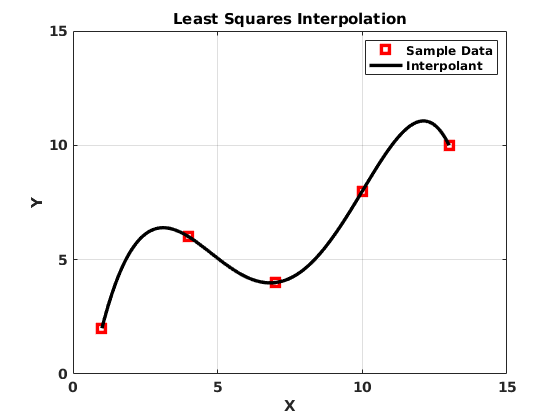
\includegraphics{lec15n-ex-ls-interp.png}
\caption{Least squares interpolation of data points.}
\label{fig:lec15n-ex-ls-interp}
\end{marginfigure}
Notice that, while the interpolant---as required---manages to pass through all of the data points, it is not an altogether great representation of the overall trend of the data.\sidenote{I suspect that  you would not want to really use the interplant to estimate values between the data points.} Some other problems that are inherent to this approach:
\begin{enumerate}
\item As $n$ increases, the columns of \lstinline[style=myMatlab]{X} are more ``like'' each other.  As a result, the condition number of \lstinline[style=myMatlab]{(X'*X)} increases and, as we learned in Lecture 10, there is therefore greater numerical error in solving the linear system to find the coefficients.  In fact, when I execute this code in MATLAB, an error is issued due to the high condition number of \lstinline[style=myMatlab]{(X'*X)}:

\begin{figure}
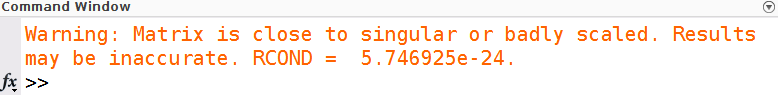
\includegraphics[width=0.75\textwidth]{lec15n-ex-ls-interp-warn.png}
\caption{Warning issued by MATLAB due to the high condition number of \lstinline[style=myMatlab]{(X'*X)}.}
\label{fig:lec15n-ex-ls-interp-warn}
\end{figure}

\item Solving a set of linear equations for the interpolating coefficients is inconvenient for some applications.  Working in a MATLAB environment we might for get that, generally speaking, solving a linear system of equations is complicated. 
\end{enumerate}

\noindent For applications later in the course, such as finite element methods, we will be very picky about the quality of interpolation functions and we will not be particularly interested in solving systems of linear equations on each domain that we hope to use such interpolations.  Luckily, there are better methods that avoid both of these problems.

\section{Lagrange Polynomial Interpolation}

Suppose we have 3 data points---$x_1$, $x_2$, and $x_3$---and we want to derive a 2\textsuperscript{nd} order polynomial interpolant, and we specify the polynomial as follows:
\begin{equation*}
f(x) = y = a_1(x-x_2)(x-x_3) + a_2(x-x_1)(x-x_3) + a_3(x-x_1)(x-x_2)
\end{equation*}
Notice the form of this polynomial; when we evaluate $f(x)$ at $x_1$, the first term on the right is the only non-zero term; when we evaluate $f(x_2)$, only the second term on the right is non-zero and similarly for when we evaluate $f(x_3)$.  This makes it easy to find values for $a_1$, $a_2$ and $a_3$.  Since
\begin{align*}
f(x_1) &= y_1 \\
&=a_1(x_1 - x_2)(x_1 - x_3) + a_2 \cancelto{0}{(x_1 - x_1)}(x_1 - x_3) + a_3\cancelto{0}{(x_1 - x_1)}(x_1 - x_2) \\
\Rightarrow a_1 &= \frac{y_1}{(x_1 - x_2)(x_1 - x_3)} 
\end{align*}
We can derive equations for $a_2$ and $a_3$ in the same way:
\begin{align*}
a_2 & = \frac{y_2}{(x_2 - x_1)(x_2 - x_3)} \\
a_3 & = \frac{y_3}{(x_3 - x_1)(x_3 - x_2)}
\end{align*}

\noindent Thus we have specified, what we will call, a Lagrange polynomial through these points:
\begin{equation*}
f(x) = \frac{(x - x_2)(x - x_3)y_1}{(x_1 - x_2)(x_1 - x_3)} + \frac{(x - x_1)(x-x_3)y_2}{(x_2 - x_1)(x_2 - x_3)} + \frac{(x - x_1)(x-x_2)y_3}{(x_3-x_1)(x_3 - x_2)}
\end{equation*}
